\section{Your first spectrum}
\label{sec:quickstart}

Two objects and two functions define the basic workflow: \texttt{SpectroscopySystem}
constructs the system, \texttt{GaussianPulse} defines a pulse,
\texttt{finite\_pulse\_spectrum} calculates the two-dimensional response,
and \texttt{plot\_spectrum} displays it.

\subsection{Copy and run the example}

The following two blocks form one complete program. Copy them, in order,
into a Python script or notebook. Only the installed package and its
standard dependencies are needed; no GitHub checkout or repository helper
is required. The example displays a figure and does not write any files.
For a script named \texttt{first\_spectrum.py}, run
\texttt{python first\_spectrum.py} from the folder containing that script.

\par\noindent
\begin{minipage}{\linewidth}
\lstinputlisting[style=python,firstline=1,lastline=36,caption={Part 1: construct the system and obtain its stationary state.},label={lst:first-spectrum}]{../../examples/manual/01_first_spectrum.py}
\end{minipage}\par

The two operators \texttt{a} and \texttt{b} lower the two-level sites.
Their energies are $1.0$ and $1.2$, with coupling $0.1$. The complete dipole
is the sum of its raising and lowering components; supplying these
components also allows the same system to be used with models that apply
the rotating-wave approximation (RWA).
Collapse operators contain square roots of the relaxation and excitation
rates. \texttt{stationary\_state()} returns a density matrix; pass that
matrix explicitly as \texttt{rho0} in the calculation.

\par\noindent
\begin{minipage}{\linewidth}
\lstinputlisting[style=python,firstline=38,lastline=66,caption={Part 2: calculate and display the spectrum.}]{../../examples/manual/01_first_spectrum.py}
\end{minipage}\par

The same pulse is used for all three interactions. Its \texttt{sigma}
is the standard deviation of the Gaussian field envelope. With
$\hbar=1$, frequencies and rates are in inverse model time units;
\texttt{sigma} and the waiting time \texttt{T} use model time units.
\texttt{pathway="NR"} selects the nonrephasing convention.
Positive \texttt{eta} ensures causal-transform convergence and adds
broadening; Section~\ref{sec:linear} explains its choice.

The result is a complex array with shape
$(\mathrm{len}(\omega_3),\mathrm{len}(\omega_1))$:
\texttt{S[j, i]} corresponds to \texttt{omega3[j]} and
\texttt{omega1[i]}. Here the shape is $(31,31)$.
\texttt{component="imag"} selects the imaginary part for display;
\texttt{normalize=True} divides that displayed component by its maximum
absolute value. The complex array \texttt{S} remains available for further
calculations.

\begin{figure}[!htbp]
\centering
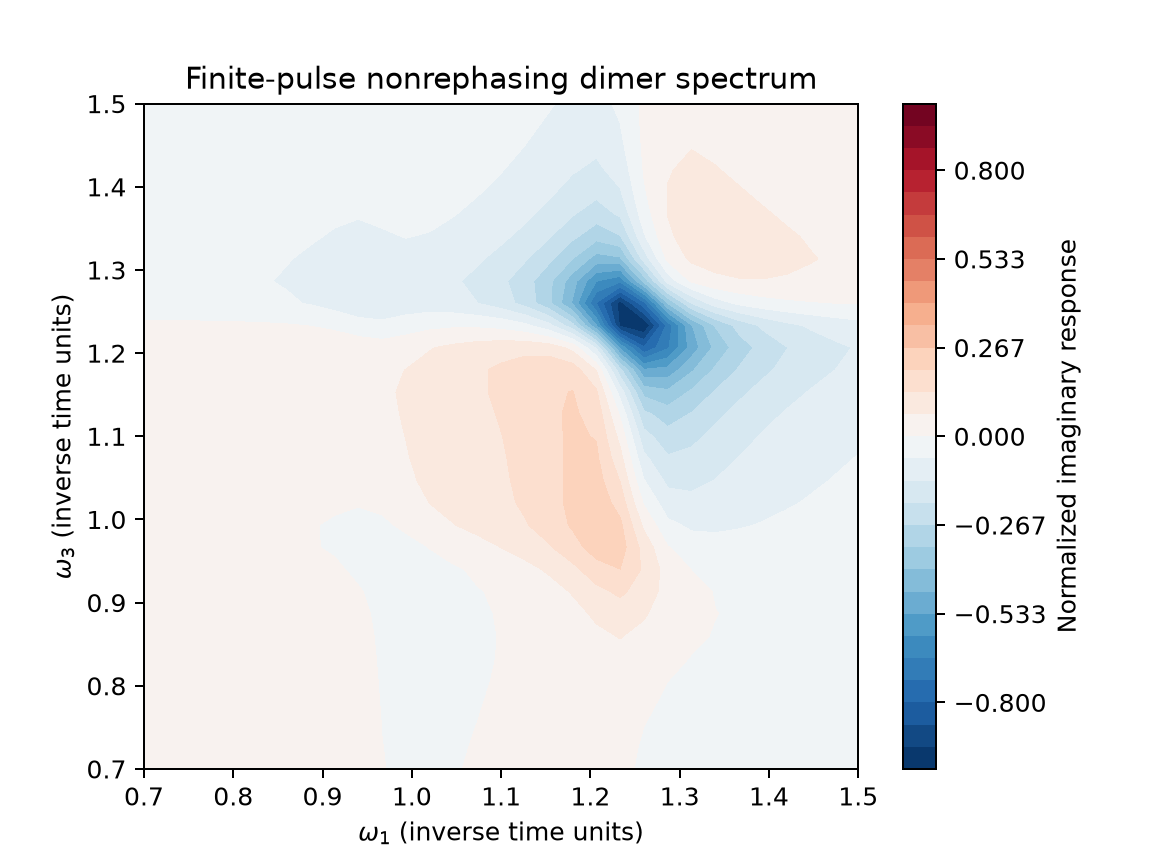
\includegraphics[width=0.78\linewidth]{figures/first_nr_spectrum.png}
\caption{Output of the first example: normalized imaginary nonrephasing
response on a $31\times31$ frequency grid. The horizontal coordinate is
$\omega_1$ and the vertical coordinate is $\omega_3$, both in inverse model
time units. The color scale shows the signed imaginary response.}
\label{fig:first-spectrum}
\end{figure}

\subsection{Choose a model}
\label{sec:models-at-a-glance}

Five functions calculate third-order spectra on the same type of
frequency grid. The RWA retains resonant raising and lowering interactions. The first four models form
an approximation ladder; the full impulsive function is an additional
molecular reference.

\begin{longtable}{@{}p{0.49\linewidth}p{0.45\linewidth}@{}}
\toprule
\textbf{Function} & \textbf{Calculation} \\
\midrule
\endhead
\texttt{finite\_pulse\_spectrum} (A) &
Full interaction with finite Gaussian pulse dressing. \\
\texttt{finite\_pulse\_rwa\_spectrum} (B) &
Finite Gaussian pulse dressing with RWA interactions. \\
\texttt{short\_pulse\_rwa\_spectrum} (C) &
RWA molecular response multiplied by scalar Gaussian spectral envelopes. \\
\texttt{impulsive\_rwa\_spectrum} (D) &
RWA molecular response without pulse filtering or field prefactors. \\
\texttt{impulsive\_spectrum} &
Full-interaction molecular response without pulses or an R/NR selector. \\
\bottomrule
\end{longtable}

To use B or C in the first example, replace the spectrum function with
one of the following, keeping the same arguments:
\begin{itemize}
\item \texttt{pulsus.finite\_pulse\_rwa\_spectrum}
\item \texttt{pulsus.short\_pulse\_rwa\_spectrum}
\end{itemize}
The example already supplies the dipole components required by the RWA.
For D, omit the three pulse arguments:
\begin{lstlisting}[style=python]
S = pulsus.impulsive_rwa_spectrum(
    system=system,
    omega1=omega1, omega3=omega3,
    T=20.0, eta=0.02,
    pathway="NR", rho0=rho_ss,
)
\end{lstlisting}
For the full impulsive model, use \texttt{pulsus.impulsive\_spectrum}
and also omit \texttt{pathway}. Impulsive functions return a molecular
response without the Gaussian field factors, so their absolute amplitudes
are not on the same scale as the finite-pulse calculation.

For a one-dimensional spectrum, use a linear spectrum function.
Section~\ref{sec:linear} introduces the four linear models and their
calling patterns. Section~\ref{sec:third-order} develops
the third-order models and R/NR conventions in more detail.
